\documentclass{innosoft}
\begin{document}
%
% Detalles del artículo, título y autores
\def\tipoarticulo{Art\'iculos originales} % Artículos originales | Artículos de revisión | Artículos cortos
\def\tematica{Ingenier\'ia de software} % Ingeniería de software | Gestión de software | Calidad de software | Técnicas de programación | Programación paralela y distribuida | Tecnologías de bases de datos | Inteligencia artificial | Procesamiento de imágenes | Reconocimiento de patrones | Redes y seguridad informática | Tecnologías de la información y las comunicaciones | Desarrollo de aplicaciones informáticas

\def\doi{10.48168/innosoft.sXX.aXXX}
\def\ark{ark:/42411/sXX/aXXX}

\def\volume{x}
\def\no{x}
\def\month{x-y}
\def\year{z}
\def\pages{x-y}

\setcounter{page}{1}

\title{T\'itulo en espa\~nol (Times New Roman, negritas, 18 puntos, no exceder las 15 palabras)}
\def\englistitle{T\'itulo en ingl\'es (Times New Roman, negritas, cursiva, 18 puntos)}
\author[1\orcidID{0000-1111-2222-3333}*]{\bf Nombre y apellidos}
\author[2\orcidID{1111-1111-2222-3333}]{\bf Nombre y apellidos}
\author[3\orcidID{1234-1111-2222-3333}]{\bf Nombre y apellidos} 

\affil[1]{Afiliaci\'on institucional completa. Direcci\'on postal.  \href{mailto:correo@dominio.com}{\nolinkurl{correo@dominio.com}}}
\affil[2]{Afiliaci\'on institucional completa. Direcci\'on postal.  \href{mailto:correo@dominio.com}{\nolinkurl{correo@dominio.com}}}
\affil[3]{Afiliaci\'on institucional completa. Direcci\'on postal.  \href{mailto:correo@dominio.com}{\nolinkurl{correo@dominio.com}}}
\def\authormail{\href{mailto:correo@dominio.com}{\nolinkurl{correo@dominio.com}}
}
%
%
\maketitle
\begin{abstract}
\par\noindent
\vskip -1em
En un solo p\'arrafo (Times New Roman, 11 puntos). El resumen tiene como objetivo orientar al lector a identificar el contenido b\'asico de forma r\'apida y exacta y a determinar la relevancia del contenido. Debe redactarse en tercera persona, en tiempo pasado exceptuando la frase concluyente, ser claro, descriptivo y poseer 250 palabras como m\'aximo, contener los objetivos del trabajo, la metodolog\'ia utilizada y los resultados alcanzados y finalizar con un comentario respecto al significado de los resultados o una peque\~na conclusi\'on. No debe incluir referencias, abreviaturas ni ecuaciones.
\vskip 1em
\keywords{Palabra 1, Palabra 2, Palabra 3, Palabra 4, Palabras 5 (Times New Roman, 11 puntos)
Entre 3 y 5 palabras clave ordenadas alfab\'eticamente, las cuales deben reflejar el contenido central del trabajo y ayudar a indizar el art\'iculo.}
\vskip 1em
\englishabstract{En un solo p\'arrafo y hasta 250 palabras (Times New Roman, cursiva, 11 puntos)}
\vskip 1em
\englishkeywords{Palabra 1, Palabra 2, Palabra 3, Palabra 4, Palabras 5 (Times New Roman, cursiva, 11 puntos)}
\end{abstract}

\onehalfspacing
\parskip=12pt
\section*{Introducci\'on}
Los autores deben respetar y cumplir rigurosamente con las normas y formato de publicaci\'on de la Revista de Innovaci\'on y Software. Para ello, se recomienda que el autor siga estas instrucciones, como modelo para la entrega de su art\'iculo, debe respetar tipos de letra, interlineados, m\'argenes y dem\'as caracter\'isticas de formato establecidas en esta plantilla. Se debe escribir en tercera persona (En este trabajo se describen, se presenta, se eval\'ua, se emplearon, etc.).
El estilo de redacci\'on deber\'a ser directo y t\'ecnico; s\'olo se permite el empleo de t\'erminos redundantes cuando el uso de sin\'onimos lesione la claridad o precisi\'on del escrito. Se enfatiza el uso correcto de la puntuaci\'on; el uso de frases cortas puede ayudar a mejorar la claridad del art\'iculo. Para las unidades se deber\'a emplear el sistema internacional de unidades. As\'i mismo, se deber\'an definir las abreviaturas y siglas la primera vez que aparezcan en el texto. Las ecuaciones y dem\'as expresiones num\'ericas deber\'an estar numeradas en secuencia.
Los p\'arrafos se escribir\'an en Times New Roman a 11 puntos y con espaciado 1,5 y una l\'inea en blanco como separador.
La introducci\'on constituye una presentaci\'on del tema y debe incluir los objetivos trazados, exponer brevemente los trabajos m\'as relevantes y destacar las contribuciones de otros autores al tema objeto de estudio, as\'i como justificar las razones por las que se realiza la investigaci\'on. 


\section*{Materiales y m\'etodos o Metodolog\'ia computacional}\label{metodos}

Los p\'arrafos se escribir\'an en Times New Roman a 11 puntos y con espaciado 1,5 y una l\'inea en blanco como separador. En esta secci\'on se explica c\'omo se hizo la investigaci\'on. Se describe el dise\~no de la misma y se explica c\'omo se llev\'o a la pr\'actica, justificando la elecci\'on de m\'etodos y t\'ecnicas de forma tal que un lector pueda repetir el estudio.

\subsection*{Subep\'igrafes en caso de utilizarse}

Los p\'arrafos se escribir\'an en Times New Roman a 11 puntos y con espaciado 1,5 y una l\'inea en blanco como separador.


\section*{Resultados y discusi\'on}

Los p\'arrafos se escribir\'an en Times New Roman a 11 puntos y con espaciado 1,5 y una l\'inea en blanco como separador. Los resultados obtenidos se exponen despu\'es de explicar las t\'ecnicas seleccionadas y descritas en la secci\'on anterior. Se incluyen las tablas y figuras que expresan de forma clara los resultados del estudio realizado por el investigador sin que repitan lo indicado en el texto. M\'as que la soluci\'on t\'ecnica expuesta se espera encontrar aquellos elementos que hacen que lo realizado constituya una novedad o una mejora en su campo de acci\'on y su superioridad con respecto a soluciones similares. En la discusi\'on se presenta el an\'alisis de los resultados obtenidos que deben corresponder a los objetivos planteados en el art\'iculo. Se utilizar\'a el editor de ecuaciones para generar las distintas f\'ormulas y ecuaciones que se presentar\'an en el art\'iculo, enumer\'andolas en el orden que aparezcan.

\begin{equation}
\binom{n}{k} = \frac{n!}{k!(n-k)!}
\end{equation}\\
Para referirse a una ecuaci\'on en el texto podr\'a hacerse de la siguiente manera: La Ecuaci\'on 1 muestra ... o El \'indice de elasticidad se describe en la Ecuaci\'on 1.\\
\begin{equation}
\sum_{n=1}^{\infty} 2^{-n} = 1
\end{equation}
\begin{figure}
\begin{center}
	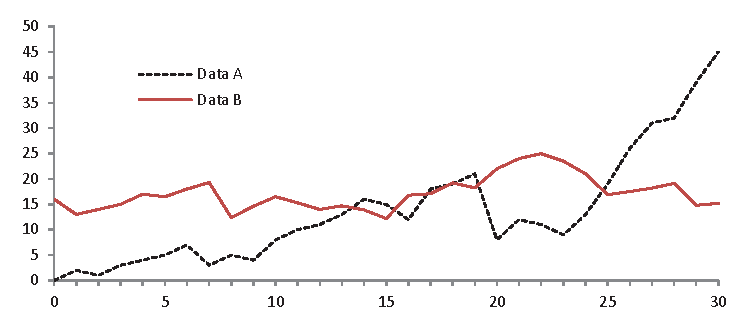
\includegraphics[width=0.9\textwidth]{fig1.eps}
\end{center}
\caption{El t\'itulo de las figuras se colocar\'a en la parte inferior, centrado, utilizando numeraci\'on secuencial seg\'un el orden en que aparecen en el trabajo.}
\end{figure}

\begin{table*}[!ht]
\centering
\caption{El t\'itulo de las tablas en la parte superior, centrado, utilizando 
numeraci\'on secuencial seg\'un el orden en que aparecen en el trabajo.}
\label{tab:actions_classification} 
\begin{threeparttable}[b]
\begin{tabular}{|p{4cm}|p{4cm}|p{4cm}|p{4cm}|}
	\hline 
	\textbf{} & \textbf{Columna 1} & \textbf{Columna 2} & \textbf{Columna 
3}\\
	\hline 
	\textbf{Fila 1} & x\tnote{a}  & y & z\\
	\hline 
	\textbf{Fila 2} & x  & y & z\tnote{b}\\
	\hline
\end{tabular}
\begin{tablenotes}
\item [a] De emplear notas aclaratorias se colocar\'an al pie de la tabla.\\
\item [b] Otra nota aclaratoria.
\end{tablenotes}
\end{threeparttable}
\end{table*}



\section*{Conclusiones}

Los p\'arrafos se escribir\'an en Times New Roman a 11 puntos y con espaciado 1,5 y una l\'inea en blanco como separador. Las conclusiones se derivan del trabajo realizado. Toda conclusi\'on debe estar fundamentada en lo expuesto y discutido en el trabajo y debe reflejar el cumplimiento de los objetivos. Deben indicar c\'omo el trabajo contribuye o es un avance en el campo y objeto de estudio. Adem\'as deben sugerir usos y trabajos futuros.


\section*{Agradecimientos (Opcional)}
Los p\'arrafos se escribir\'an en Times New Roman a 11 puntos y con espaciado 1,5 y una l\'inea en blanco como separador. Se a\~naden los nombres de personas que contribuyeron a la investigaci\'on pero que no se consideran como parte del colectivo de autores. Se incluyen los nombres de instituciones o proyectos que proporcionaron facilidades para la realizaci\'on de la investigaci\'on tanto materiales, log\'isticas o financieras.

\section*{Contribuci\'on de Autor\'ia}
Los p\'arrafos se escribir\'an en Times New Roman a 11 puntos y con espaciado 1,5 y una l\'inea en blanco como separador. Se a\~naden los nombres de los autores de la investigaci\'on seguido de los roles de autor\'ia que cada autor desarroll\'o. 

Nombre completo del Autor 1: \href{http://credit.niso.org/contributor-roles/conceptualization/}{Conceptualizaci\'on}, \href{http://credit.niso.org/contributor-roles/investigation/}{Investigaci\'on}, \href{http://credit.niso.org/contributor-roles/methodology/}{Metodolog\'ia}, \href{http://credit.niso.org/contributor-roles/software/}{Software}, \href{http://credit.niso.org/contributor-roles/validation/}{Validaci\'on}, \href{http://credit.niso.org/contributor-roles/writing-original-draft/}{Redacci\'on - borrador original}. Nombre Completo del Autor 2: \href{http://credit.niso.org/contributor-roles/conceptualization/}{Conceptualizaci\'on}, \href{http://credit.niso.org/contributor-roles/investigation/}{Investigaci\'on}, \href{http://credit.niso.org/contributor-roles/methodology/}{Metodolog\'ia},  \href{http://credit.niso.org/contributor-roles/formal-analysis/}{An\'alisis formal},  \href{http://credit.niso.org/contributor-roles/resources/}{Recursos}, \href{http://credit.niso.org/contributor-roles/visualization/}{Visualizaci\'on}, \href{http://credit.niso.org/contributor-roles/supervision/}{Supervisi\'on}, \href{http://credit.niso.org/contributor-roles/project-administration/}{Administraci\'on de proyectos}, \href{http://credit.niso.org/contributor-roles/funding-acquisition/}{Adquisici\'on de fondos}, \href{http://credit.niso.org/contributor-roles/data-curation/}{Curaci\'on de datos}, \href{http://credit.niso.org/contributor-roles/writing-review-editing/}{Escritura, revisi\'on y edici\'on}.

\section*{Informaci\'on sobre las Referencias (Eliminar secci\'on)}

En el cuerpo del art\'iculo se deben citar las referencias de manera num\'erica de acuerdo al manual de estilo IEEE (\url{http://ieeeauthorcenter.ieee.org/wp-content/uploads/IEEE-Reference-Guide.pdf}). A continuaci\'on de la frase citada se utiliza una numeraci\'on secuencial dentro de corchetes, despu\'es de un espacio, en la misma l\'inea de texto y antes de cualquier tipo de puntuaci\'on. Cada n\'umero se corresponde con una referencia que contenga informaci\'on de la fuente citada. Las citas est\'an numeradas en el orden en que aparecen. Una vez que se ha citado una fuente, se utiliza el mismo n\'umero en todas las referencias posteriores en el informe. No se hace distinci\'on entre fuentes electr\'onicas e impresas, excepto en los detalles de referencia de la cita.\\\\
Ejemplos:

``...end of the line for my research [13].''\\
``La teor\'ia fue planteado por primera vez en 1987 [1].''\\
``Scholtz [2] ha sugerido ...''\\
``Por ejemplo, ver [7].''\\
``Varios estudios [3, 4, 15, 22] han sugerido que ...''

No es necesario escribir ``en la referencia [2]''. Simplemente escriba ``en [2]''. El m\'etodo preferido para citar m\'as de una fuente a la vez es enumerar cada referencia en sus propios corchetes, luego separarlos con una coma o gui\'on:

[1], [3], [5]\newline
[1] -- [5]

Los siguientes ejemplos muestran el formato para una variedad de fuentes electr\'onicas e impresas. Estas citas son las de mayor uso, el listado completo puede encontrarse en (\url{http://ieeeauthorcenter.ieee.org/wp-content/uploads/IEEE-Reference-Guide.pdf}).

Libros de una serie \cite{IEEEexample:incollectionwithseries}, P\'aginas de un libro \cite{IEEEexample:inbookpagesnote}, Libro con editor \cite{IEEEexample:bookwitheditor}, Libro de una serie con volumen \cite{IEEEexample:bookwithseriesvolume}, P\'aginas de un art\'iculo \cite{IEEEexample:articlelargepages}, Libro con muchos autores \cite{IEEEexample:incollectionmanyauthors}, Libro de un autor repetido \cite{IEEEexample:repeatedauthorone}, Libro del mismo autor \cite{IEEEexample:repeatedauthortwo}, Libro com\'un \cite{IEEEexample:book_typical}, \cite{IEEEexample:book}, \cite{IEEEexample:inbook}, Art\'iculo sin publicar \cite{IEEEexample:TBPmisc}, Art\'iculo presentado en congreso \cite{IEEEexample:presentedatconf}, \cite{IEEEexample:articledualmonths}, Manual \cite{IEEEexample:motmanual}, Patente \cite{IEEEexample:uspat}, \cite{IEEEexample:jppat}, \cite{IEEEexample:frenchpatreq}, Reporte t\'ecnico \cite{IEEEexample:techreptype}, \cite{IEEEexample:techrepstdsub}, \cite{IEEEexample:techrep}, \cite{IEEEexample:techreptypeii}, Tesis \cite{IEEEexample:phdurl}, \cite{IEEEexample:masterstype}, \cite{IEEEexample:masters}, Est\'andar \cite{IEEEexample:standard}, Sitio web \cite{IEEEexample:electronhowinfo}, \cite{IEEEexample:electronorgadd}, \cite{IEEEexample:electronhowinfo2}, Cap\'itulo de libro \cite{IEEEexample:incollection_chpp}, Peri\'odico \cite{IEEEexample:periodical}.  

\bibliographystyle{IEEEtran}
\bibliography{referencias}


\end{document}